\documentclass{article}
\usepackage[utf8]{inputenc}
\usepackage[top=2cm, bottom=2cm, left=4cm, right=4cm]{geometry}
\title{Rapport de TP - MongoDB}
\author{loïc divad}
\date{December 2014}
\usepackage[T1]{fontenc}
\usepackage{lineno}
\usepackage{natbib}
\usepackage{graphicx}
\usepackage{hyperref}
\usepackage{enumitem}
\usepackage{wrapfig}
\usepackage{tabularx}


\newenvironment{block}[1]{\par\vspace{5pt}\emph{#1:}} {\par\vspace{5pt}}

\usepackage{listings}
\usepackage{color}
\usepackage[usenames,dvipsnames]{xcolor}

\lstdefinelanguage{JavaScript}{
  keywords={typeof, new, true, false, catch, function,  null, catch, switch, var, if, in, while, do, else, case, break},
  keywordstyle=\color{cyan}\bfseries,
  ndkeywords={class, return, export, boolean, throw, implements, import, this},
  ndkeywordstyle=\color{Blue}\bfseries,
  identifierstyle=\color{black},
  sensitive=false,
  comment=[l]{//},
  morecomment=[s]{/*}{*/},
  commentstyle=\color{Plum}\ttfamily,
  stringstyle=\color{OliveGreen}\ttfamily,
  morestring=[b]',
  morestring=[b]",
  numbers=left
}

\lstset{
   language=JavaScript,
   extendedchars=true,
   basicstyle=\footnotesize\ttfamily,
   showstringspaces=false,
   showspaces=false,
   numbers=left,
   numberstyle=\footnotesize,
   numbersep=9pt,
   tabsize=2,
   breaklines=true,
   showtabs=false,
   captionpos=b
}

\usepackage{listings}
\usepackage{color}

\lstdefinelanguage{JSON}{
  keywords={typeof, new, true, false, catch, function, return, null, catch, switch, var, if, in, while, do, else, case, break},
  keywordstyle=\bfseries,
  ndkeywords={class, export, boolean, throw, implements, import, this},
  ndkeywordstyle=\bfseries,
  identifierstyle=\color{black},
  sensitive=false,
  comment=[l]{//},
  morecomment=[s]{/*}{*/},
  commentstyle=\ttfamily,
  stringstyle=\ttfamily,
  morestring=[b]',
  morestring=[b]",
  numbers=none,
}

\lstset{
   language=JSON,
   extendedchars=true,
   basicstyle=\footnotesize\ttfamily,
   showstringspaces=false,
   showspaces=false,
   %numberstyle=\footnotesize,
   %numbersep=9pt,
   tabsize=2,
   breaklines=true,
   showtabs=false,
   captionpos=b
}



\usepackage{listings}
\usepackage{color}
\usepackage[usenames,dvipsnames]{xcolor}

\lstdefinelanguage{Mongo}{
  basicstyle=\footnotesize\ttfamily,
  keywords={typeof, new, true, false, catch, function,  null, catch, switch, var, if, in, while, do, else, case, break, collection},
  keywordstyle=\color{cyan}\bfseries,
  ndkeywords={class, return, export, boolean, throw, implements, import, this, db},
  ndkeywordstyle=\color{blue}\bfseries,
  identifierstyle=\color{black},
  sensitive=false,
  comment=[l]{//},
  morecomment=[s]{/*}{*/},
  commentstyle=\color{Plum}\ttfamily,
  stringstyle=\color{OliveGreen}\ttfamily,
  morestring=[b]',
  morestring=[b]",
  numbers=left
}

\lstset{
   language=Mongo,
   extendedchars=true,
   basicstyle=\footnotesize\ttfamily,
   showstringspaces=false,
   showspaces=false,
   numbers=left,
   numberstyle=\color{black}\footnotesize,
   numbersep=9pt,
   tabsize=2,
   breaklines=true,
   showtabs=false,
   captionpos=b
}


\subsection*{Map / Reduce avec Pymongo\textsuperscript{11}}

\par Pymongo est une dépendence python qui permet de s'adrésser à mogodb. Une fois L'instence mongo lancée L'import de ce module permet la connection et donne accès à des fonctions mongo.

\begin{tt} >>>>>> Import mongo\end{tt}

\par Pour faire un exemple on propose de reprendre la fonction map reduce de pymongo appliquée à la base de lapin de la partie 9. Pour lancer le script:

\begin{tt} > python mapredbunny.py\end{tt}

\lstset{language=python}
\begin{lstlisting}
##########################################################
#     EXEMPLE DE MAP / REDUCE SUR MONGODB                #
##########################################################

# Import du connecteur et du traducteur bson #
import pymongo
from bson.code import Code # Traduction du code Js compris par mongodb #

# Connection a la bonne BDD #
db = pymongo.MongoClient().lapins 

# ecriture du mappeur #
mapp = Code(""" 
            function() {
                this.regime.forEach(function(r){
                    emit(r,1);
                });
            }
            """)

# ecriture du reduceur #
red = Code(""" 
            function(key, tab) {
                var sum = 0;
                for(var i; i < tab.length - 1; i++){
                    sum += values[i];
                }
                return sum;
            }

            """)

# Lancement de l'agregation #
res = db.france.map_reduce(mapp, red, "mapred_bunny", query={"genre":"h"})
#
Le resultat est disponible
dans la collection "mapred_bunny"
#
\end{lstlisting}

\par La collection retour est une suite de document contenant: un nom d'alliment et le nombre de lapins mâles qui en mange. Ce n'est pas très util car ce n'est qu'un exemple. Il faut s'imaginer que la donnée est maintenant bien agrégée pour réaliser de super grafiques sur le régime des lapins de la collection france.

{\let\thefootnote\relax\footnotetext{\textsuperscript{11} \textit{{\href{http://api.mongodb.org/python/current/?_ga=1.152073017.1419368140.1410728889}{ API du connecteur "pymongo"}.}}}


\begin{document}

\maketitle

\section{Introduction}
Ce TP est associé aux cours électifs de deuxième année et porte sur la base de donnée NoSQL orientée documents, MogoDB. Elle diffère en quelques points avec les outils habituellement utilisés par les DBA tel que les bases ORACLE vu dans le cours de base de donnée avancée. Ne pouvant assiter au cours je rédige ici une partie du TP.


\section{Requêtage}
    
    \begin{itemize}
        \item \begin{tt} db.media.find() \end{tt} \newline
        Cette requête trouve tous les éléments de la collection "media". Cette collection appartient à la base de donnée "library".

        \item \begin{tt} db.media.find(\{Artist:"Nirvana"\}) \end{tt} \newline
        Cette requête trouve tous les documents ayant pour valeur "Nirvana" associée à leur champ artiste.
        
        \item \begin{tt} db.media.find(\{Artist:"Nirvana"\},\{Title: 1\}) \end{tt} \newline
        Cette requête trouve tous les documents ayant pour valeur "Nirvana" dans leur champ artiste et n'affiche que le champ "Title" et "\_id" grâce à une projection\textsuperscript{1}.
        
        \item \begin{tt} db.media.find(\{Artist:"Nirvana"\},\{Title:0\}) \end{tt} \newline
        Cette requête trouve tous les documents ayant pour valeur "Nirvana" dans leur champ artiste sans afficher leur champ "title".
        
        \item \begin{tt} db.media.find(\{"Tracklist.Title":"In Bloom"\}) \end{tt} \newline
        Cette requête trouve tous les documents ayant un sous document de titre "in Bloom".

        \item \begin{tt} db.media.findOne() \end{tt} \newline
        findOne retourne le premier document respectant les conditions passées en paramètre (aucune conditions dans ce cas). Elle renvoie donc le premier document inséré dans la collection.

    \end{itemize}
    
    \begin{block}{Note}
         La projection\textsuperscript{1} est le deuxième argument optionel de la méthode .find() il est de forme "field": 1/0 et permet de spécifier les champs que l'on veut récupérer. Par défaut le champ \_id s'affiche si on ne préscise pas {"\_id": 0} 
    \end{block}

{\let\thefootnote\relax\footnotetext{\textsuperscript{1}\textit{Usages and examples of \href{http://docs.mongodb.org/manual/reference/operator/projection/positional/}{\$(projection)}}}}

    \begin{itemize}
        \item \begin{tt} db.media.find().sort(\{Title:1\}) \end{tt} \newline
        La méthode .find() retourne un objet de type "Object Cursor". En applicant la méthode sort on ordonne le résultat de la requête. Ici on affiche tous les documents de la collection media dans la base Library par ordre croissant. 
        \item \begin{tt} db.media.find().sort(\{Title:-1\}) \end{tt} \newline
        Ici on affiche tous les documents de la collection media dans la base Library par ordre décroissant.
        \item \begin{tt} db.media.find().limit(10) \end{tt} \newline
        Ici on affiche les 10 premiers documents de la collection.
        
        \item \begin{tt} db.media.find().pretty() \end{tt} \newline
        La commande .pretty() permet d'agencer le JSON qui résulte de la requête pour une meilleur comprehension du résultat.
    \end{itemize}
    
    \begin{figure}[h!]
    \centering
    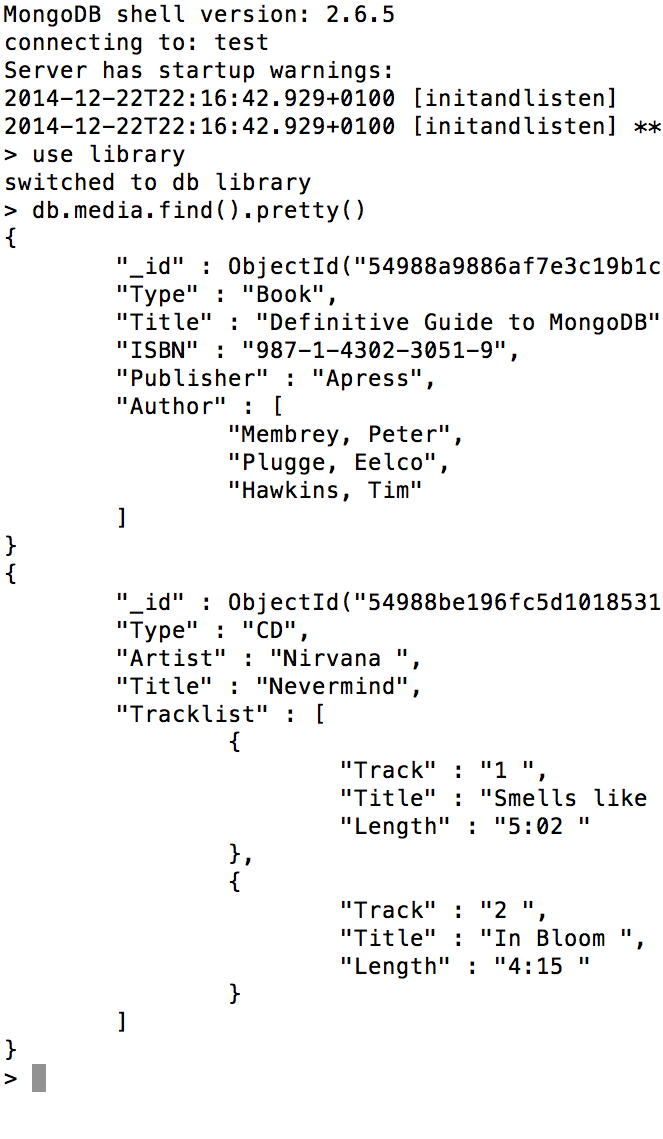
\includegraphics[scale=0.6]{img/pretty.png}
    \caption{Exemple d'utilisation de la méthode .pretty() en console}
    \end{figure}
    
    \par
        Ce comportement est automatiquement géré par l'interface RoboMongo\textsuperscript{2}. Après cette première partie sur les requêtes nous continurons le TP sur RoboMongo et laisseront tomber la consol.   

{\let\thefootnote\relax\footnotetext{\textsuperscript{2} \textit{RobotMongo, the MongoDB management tool. \href{http://robomongo.org}{http://robomongo.org}}}}
    \begin{itemize}
        \item \begin{tt} db.media.find().skip(20) \end{tt} \newline
        On recupère tous les documents à partir du 20 éléments du curseur renvoyé par .find(). La méthode .skip(n) permet de d'ignorer un certain nombre de résultats.
        \item \begin{tt} db.media.find().sort (\{Title:-1\}).limit(10).skip(20) \end{tt} \newline
        On obtient les 10 résultats à partir du 20ème sur la liste des documents par ordre décroissant des titres.
    \end{itemize}
    \begin{block}{Remarque}
        On peut trouver cette dernière requête particulièrement contre intuitive. on pourrait penser que db.media.find().sort(\{Title:-1\}).limit(m) renvoie une liste de m éléments et que l'on y applique .skip(n) pour passer les n premiers. Au lieu de celà on peut inverser les instructions .limite() et .skip(), on a le même résultat.
    \end{block}
    
    
\section{Agregation}

    \begin{itemize}
        \item \begin{tt} db.media.count() \end{tt} \newline
        Compte le nombre de documents dans la collection.
        \item \begin{tt} db.media.find(\{Publisher:"Apress",Type:"Book"\}).count()\end{tt} \newline
        Compte le nombre de documents de type livre ET d’éditeur Apresss.
        \item \begin{tt} db.media.find(\{Publisher:"Apress",Type:"Book"\}).skip(2).count(true) \end{tt} \newline
        Compte le nombre de documents de type livre ET d’éditeur Apresss sans compter les deux premiers resultats.
    \end{itemize}

    
\section{Distinct et regroupement}
    
    \par Après un bref passage par la documentation\textsuperscript{3} on sait que la méthode .disctinct() s'applique sur un objet de type collection et renvoie dans un tableau de valeurs distinctes correspondants au champ passé en paramètre de la méthode. \begin{tt} db.media.distinct("ISBN") \end{tt} renvoie alors une liste d"ISBN tous différents. La taille du tableau est également égale au nombre de livre car l"ISBN est unique.
    
    \begin{figure}[h!]
    \centering
    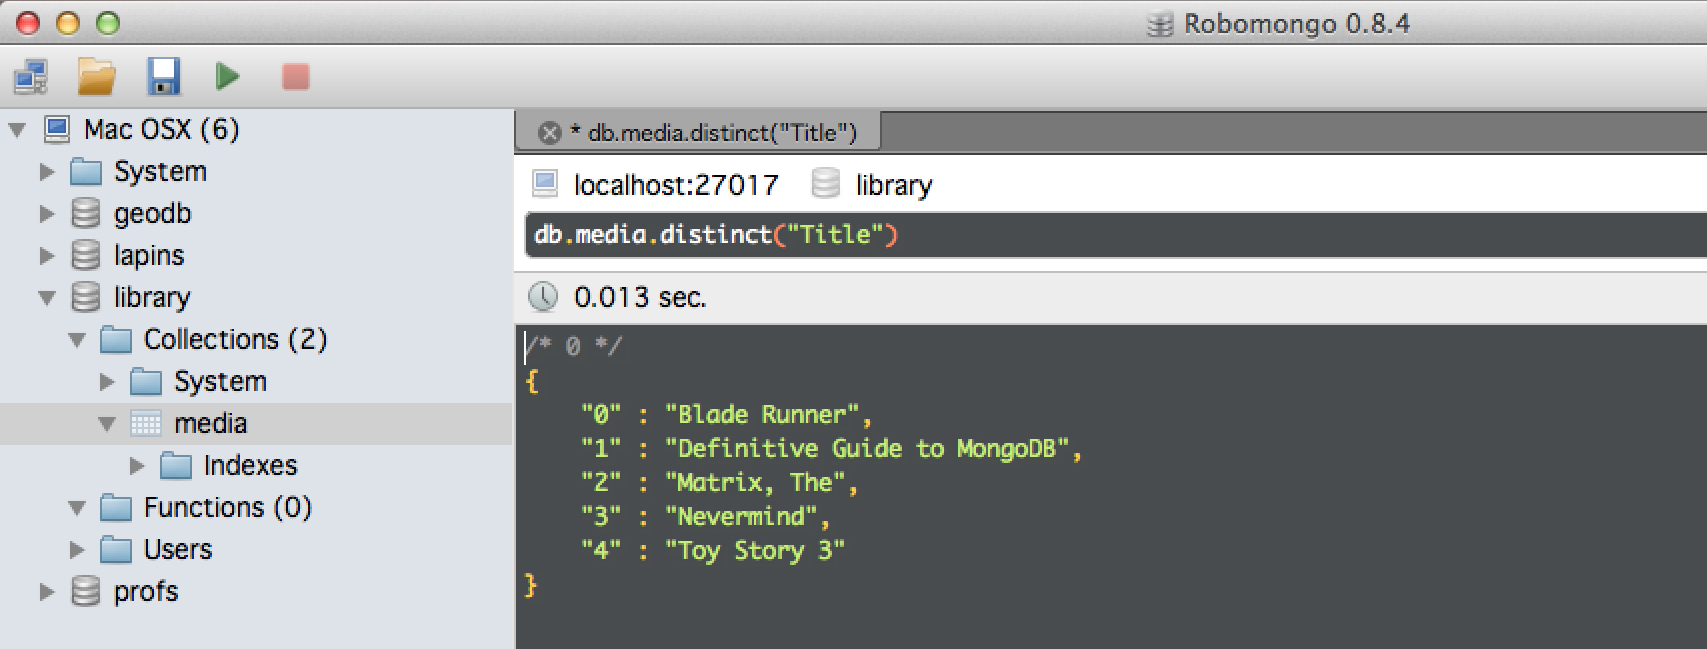
\includegraphics[scale=0.5]{img/distinct.png}
    \caption{Aperçu du tableau Javascripte retourné par la méthode .distinct()}
    \end{figure}
    
    \par Il est également possible de filtrer les documents traités par un .distinct() à l'aide d'un argument optionnel \textbf{query}. La requête suivente contruit alors un tableau de titre distinct uniquement à partir des livres de prix supérieur à 5.\newline
    
    \begin{tt} db.media.distinct("Title",\{price:\{\$gt:5\}\})\end{tt} \newline
    A l'aide des indications sur la méthode .groupe() on essaie de résoudre l'exercice suivant:
    
    \subsection{Exercice, transformer cette requête SQL en requête mongo}
    
    select a,b,sum(c) csum from coll where active=1 group by a,b \newline \newline
    \begin{tt} db.coll.group(\{ key: \{a: true, b: true\},\newline
    \indent cond: \{ active: 1 \}, \newline
    \indent reduce: function(curr, result)\{ \newline
    \indent \indent result.csum += curr.c; \newline
    \indent\}, \newline
    initial: \{csum: 0\} \newline
    \}); \newline \end{tt}
    
{\let\thefootnote\relax\footnotetext{\textsuperscript{3}\textit{\href{http://docs.mongodb.org/manual/reference/method/db.collection.distinct/}{Examples of the db.collection.distinct() method:}}}}

    
\section{Opérateur de comparaison}

    \begin{itemize}
    \item \begin{tt} db.media.find(\{Released:\{\$gt:2000\}\},\{"Cast":0\}) \end{tt} \newline
    Renvoie tous les éléments réalisés après l"an 2000 sans afficher leur casting.
    \item \begin{tt} db.media.find(\{Released:\{\$gte:1990,\$lt:2010\}\},\{"Cast":0\}) \end{tt} \newline
    Renvoie tous les documents réalisés entre 1990 et 2010.
    \item \begin{tt} db.media.find(\{Type:"Book",Author:\{\$ne:"Plugge, Eelco"\}\}) \end{tt} \newline
    Sélectionne tous les documents de type "book" dont les auteurs ne sont pas Plugge et Eelco.
    \item \begin{tt} db.media.find(\{Released:\{\$in:["1999","2008","2009"]\}\},\{"Cast":0\}) \end{tt} \newline
    Renvoie les éléments ayant une date de réalisation dans la liste suivant "\$in ".
    \item \begin{tt} db.media.find(\{Released:\{\$nin:["1999","2008","2009"]\},Type:"DVD"\},\{"Cast":0\}) \end{tt}
    Renvoie tous les dvd de 1999, 2008 et 2009.
    \item \begin{tt} db.media.find(\{\$or:[\{"Title":"Toy Story 3"\},\{"ISBN":
"987-1-4302-3051-9"\}]\}) \end{tt}
    \item \begin{tt} db.media.find(\{"Type":"DVD",\$or:[\{"Title":"Toy Story 3"\},\{"ISBN":"987-1-4302-3051-9"\}]\})
\end{tt} \newline
    \end{itemize}
    \par
    Les deux dernières requêtes renvoient les documents si le titre ou l"ISBN respecte la condition. La dernière est plus selective car elle ne concerne que les documents de type dvd. La condition "type :DVD" est en produit logique avec la condition préscédente.
    \newline
    \par 
    L'argument \textbf{\$slice} se place au sein d'une projection et peut prendre la forme d'un intervale [m,n] pour limiter les résultats de la requête. \newline
    \par 
    L'option \textbf{\$size} concerne les tableaux, c'est une condition sur le nombre délements. Ainsi la requête suivante renvoie tous les documents ayant un champ tracklist composé de 2 titres:  \begin{tt} db.media.find(\{Tracklist:\{\$size:2\}\}) \end{tt} \newline
    \par 
    L'option \textbf{\$exist} ici est assez différente de WHERE EXIST que l'on connait en SQL. Elle porte sur l'existence du champs dans un document et non sur la valeur. Le format NoSQL nous libère du traditionel schéma. Il n'y a pas de tables avec des champs obligatoires laissés à Null si une valeur est manquante. Il se peut donc que certain documents, en fonction de leur type (CD, DVD, Livre) présente ou pas certain champs comme Tracklist. La requête suivante retourne donc tous les documents susceptibles d'avoir un auteur: \begin{tt} db.media.find(\{Author:\{\$exists:true\}\}) \end{tt} \newline
    
\newpage

\section{Création d'un index}
    
    \begin{wrapfigure}[8]{l}{2.5cm}
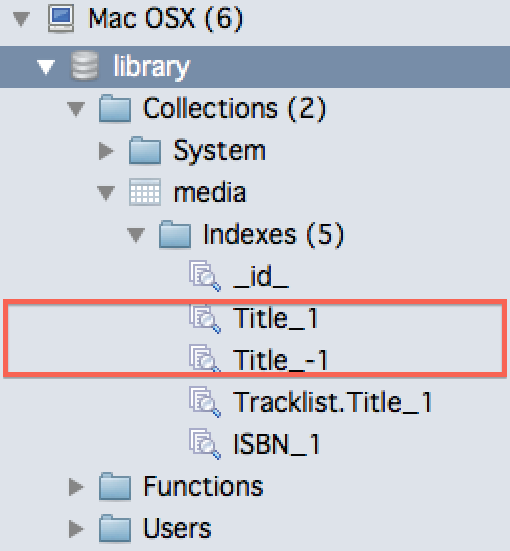
\includegraphics[scale=0.3]{img/indexes.png}
%\caption{The Universe}
\end{wrapfigure}
    \par
    Après la création de l’index avec la méthode ensureIndex un dossier arrive sous média indexes, l’index est définie au niveau de la collection associée. On y retrouve les objets index\_1 et index\_-1
    \begin{block}{Remarque}
        Sans index les recherches de type .find() ou .group() scan toute la collection. Elles font également appel, pour un large volume de data, au démon de mongodb : mongod. Ce qui est particulièrement lent. On créer alors des index pour faciliter la recherche sur les collections.
    \end{block}
    les indexes de mongodb respectent une organisation B-Tree\textsuperscript{4}… 
    \begin{block}{Note sur le model de donnée d'arbre en B}
    \newline
    C'est un model pour organiser des données de manière ordonnée. Il est sous forme d'arbre et grossit par la racine, c'est à dire que L’insertion des données (les clefs) se fait depuis le neud parent. Les clefs sont alors dirigées vers les neuds inférieures en fonction de leur valeur de sorte que le bout des branches soit ordonnée.    
    \end{block}
    \begin{figure}[h!]
    \centering
    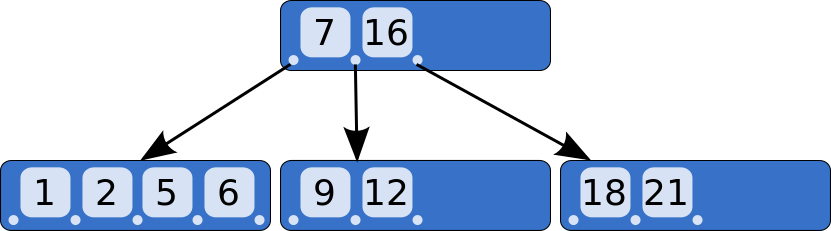
\includegraphics[scale=0.2]{img/btree.png}
    \caption{Représentation d"un arbre en B d"ordre 2.} 
    \end{figure}
    \par
    Pour faire le raprochement avec nos indexes mongodb, lindex Title\_1 correspond à la dernière ligne de l'arbre. c'est une suite de titres rangés dans l'ordre alphabétique dont chaqu'un a associé à un \_id.
    \begin{figure}[h!]
    \centering
    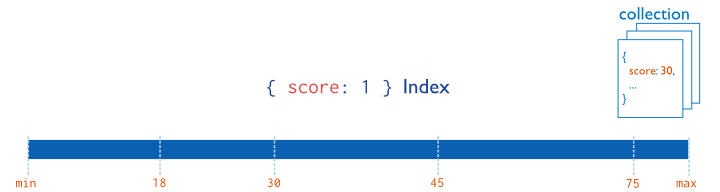
\includegraphics[scale=0.3]{img/indexmongodb.png}
    \caption{Binding entre l"index et la collection.\textsuperscript{5}}  
    \end{figure}
    \par
    La méthode .hint() force la recherche à l’aide d’un index. En indiquant des arguments on désigne un l’index approprié. Dans un premier temps lorsque l’index n’existe pas encore la ligne: \begin{tt}error:{"\$err": "bad hint", "code": 10113} \end{tt} nous indique une erreur. Une fois le l'index crée mongodb fait lien entre l'\_id indexé et le document de manière à pouvoir restituer des documents entiers.
    \begin{figure}[h!]
    \centering
    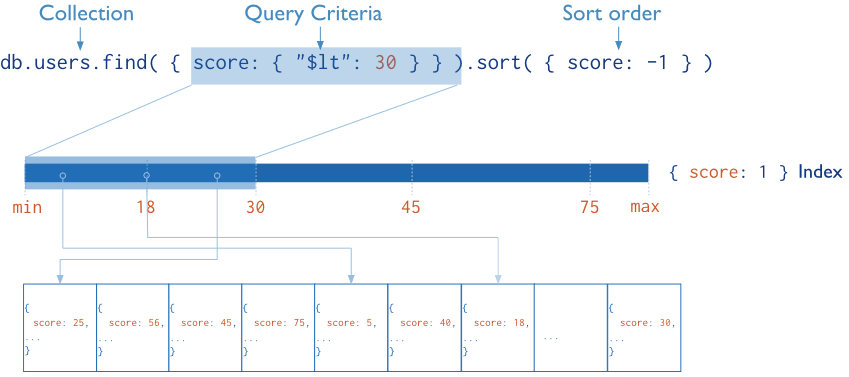
\includegraphics[scale=0.3]{img/indextocoll.png}
    \caption{Binding entre l'index et les documents de la collection\textsuperscript{5}} 
    \end{figure}

{\let\thefootnote\relax\footnotetext{\textsuperscript{4} \textit{\href{http://en.wikipedia.org/wiki/B-tree}{http://en.wikipedia.org/wiki/B-tree}}}}
        {\let\thefootnote\relax\footnotetext{\textsuperscript{5}\textit{Ressource images: \href{http://mongodb.org}{http://mongodb.org}}}}

    
\newpage

    Résultat de la méthode .getIndexes() est une liste des indexes avec les propriétés v version d’index (cette version dépend de la version de mongodb). key est le champ d’indexation, name le nom de l’index et ns pour name space, base de donnée [point] la collection.

\begin{lstlisting}[language=JSON, caption=Résultat de la méthode .getIndexes()]
{
    "0" : {
        "v" : 1,
        "key" : {
            "id" : 1
        },
        "name" : "id",
        "ns" : "library.media"
    },
    "1" : {
        "v" : 1,
        "key" : {
            "Title" : 1
        },
        "name" : "Title1",
        "ns" : "library.media"
    },
    "2" : {
        "v" : 1,
        "key" : {
            "Title" : -1
        },
        "name" : "Title -1",
        "ns" : "library.media"
    },
    "3" : {
        "v" : 1,
        "key" : {
            "Tracklist.Title" : 1
        },
        "name" : "Tracklist.Title 1",
        "ns" : "library.media"
    }
}
\end{lstlisting}
    
\section{Mise à jour des données - le U de CRUD}

        Pour faire la mise à jour d'un ou plusieur documents on a à notre disposition la fonction \textbf{.update()}. C'est une méthode d'objet collection et non celle d'un curseur renvoyé par .find() ou .group(). Cette fonction prend les arguments suivants: \textbf{query}, \textbf{object} et \textbf{option}. \newline

    \begin{lstlisting}[language=Mongo, caption=fonction update().]
db.collection.update(
    { type: "",
      size: {$gt : 30} 
    },
    {
        multi: true, // modifie tous les documents trouve par query
        upsert: true, // creer le document si il n"existe pas.
    }
);
    \end{lstlisting}

    
\newpage
    
\section{Suppression des données - le D de CRUD}
    
        Dans mongoDB la suppression peut être effectuée à différent niveaux. 
\begin{itemize}
    \item Il est possible de supprimer un document. \newline
    \begin{tt} db.media.remove(\{"Title":"Different Title"\}) \end{tt} 
    
    \item Pour vider toute une collection. \newline
    \begin{tt} db.media.remove(\{\})  \end{tt} 
  
    \item Pour supprimer une collection. \newline
    \begin{tt} db.media.drop() \end{tt} 

\end{itemize}
    
\section{Exercice i}

    L'exercice tourne autour d'une base de donnée contenant des lapins. Pour la création de la base de données et l’insertion je propose un script js qui sera joué de la façon suivante. \newline
    \begin{tt} mongo exo\_lapin.js \end{tt} \newline
    les autres requêtes seront exécutées dans le shell mongo. Après la création de la base de donnée on demande l’affichage de tous les documents\newline
    
\begin{lstlisting}[language=JavaScript, caption= Création de la base de donnée "lapin"]
var db = connect("lapins");
// Connection a la base mongo.

//creation en dure de la base.
var all_rabbits = [

  {nom: "leny", genre: "f", ville: "Lyon", regime: ["carotte",
                                                    "courgette"
                                                    ],
   poids: 4, taille: 20 },

  {nom: "bunny", genre: "h", ville: "Paris", regime: [ ],
   poids: "3", taille: ""},

  {nom: "olto", genre: "h", ville: "Paris", regime: ["raisin",
                                                     "carotte",
                                                     "salade"
                                                     ],
   poids: 5, taille: 25 }
];

// Pour charque lapin on insert une ligne du JSON
all_rabbits.forEach(function(rabbit){
  db.france.insert(rabbit);
})

print("insertion terminee.");

//affichage en console du contenut de la base.
var lapin_fr = db.france.find();

lapin_fr.forEach(function(m){
  printjson(m);
});
\end{lstlisting}
    
\newpage

    \begin{lstlisting}[language=JSON, caption= lapin.france]
~/Documents/mongo workspace loicMDIVAD \$ mongo exo_lapins.js 
MongoDB shell version: 2.6.6
connecting to: test
connecting to: lapins
insertion terminee.
{
	"_id" : ObjectId("54a025fca35fa2e9d3a4dac2"),
	"nom" : "leny",
	"genre" : "f",
	"ville" : "Lyon",
	"regime" : [
		"carotte",
		"courgette"
	],
	"poids" : 4,
	"taille" : 20
}
{
	"_id" : ObjectId("54a025fca35fa2e9d3a4dac3"),
	"nom" : "bunny",
	"genre" : "h",
	"ville" : "Paris",
	"regime" : [ ],
	"poids" : "3",
	"taille" : ""
}
{
	"_id" : ObjectId("54a025fca35fa2e9d3a4dac4"),
	"nom" : "olto",
	"genre" : "h",
	"ville" : "Paris",
	"regime" : [
		"raisin",
		"carotte",
		"salade"
	],
	"poids" : 5,
	"taille" : 25
}


\end{lstlisting}



    On applique quelques requêtes sur cette base.
\begin{itemize}
    \item Trouvez tous les lapins mâles? \newline
        \begin{tt} db.france.find(\{"genre":"m"\}); \end{tt} 
        
    \item Nombre de lapins qui aiment les carottes et qui pèsent plus de 4kg \newline
        \begin{tt} db.france.find(\{regime :\{\$all:[‘carotte’]\},poids:\{\$gt:4\}}).count();\end{tt}\newline
        Le compte donne 1, car ici on interprète plus par strictement supérieur. Si on remplace \$gt par \$gte on obtient 2.
        
    \item Les lapins qui aiment les courgettes ou les raisins ou qui n’ont pas de champ « ville »\newline
        \begin{tt} db.france.find(\{\$or:[{regime:\{\$in:["salade","courgette"]\}\},\{ville:null\}]\}); \end{tt}
        \item Tous les lapins qui n’aiment pas la salade.\newline
        \begin{tt} db.france.find(\{regime:\{\$nin:["salade"]\}\}); \end{tt} \newline
        Leny et bunny font les difficiles.
        
    \item Nous savons que Bunny se trouve en France, rajouter un champ pays à ce document.
        \begin{tt} db.france.update(\{"nom":"bunny"\},\{\$set:\{"departement":"Île-de-France"\}\}); \end{tt}
        N’ayant pas de nom de collection je l’ai appelé france. On traite donc cette question avec le nom du département.

    \item Supprimer le champ « taille », s’il existe, de tous les documents.\newline
        \begin{tt} db.france.update(\{\},\{\$unset:\{taille:""\}\},false,true); \end{tt}
        
    \item Supprimer la base de données.\newline
        \begin{tt} db.france.drop() \end{tt} \newline
        … plus de petits lapins.
    \end{itemize}
    
\section{Exercice ii - Base de donnée géographique.}
    
    On procède à l'insertion: \newline
    \begin{tt} > mongoimport -type -json -d geodb -c earthquakes --file
eartquakes.json \end{tt} \newline
    Puis on applique les modifications :
\begin{lstlisting}[language=Mongo, caption=]
db.earthquakes.find().forEach(
    function(eq){
        eq.properties.iso_date = new Date(eq.properties.time);
        db.earthquakes.save(eq);
    }
);
\end{lstlisting}

    Le sujet propose de convertir la chaîne de caractère du champ properties.types en tableau et le mettre dans un champ types\_as\_array.
    
    \begin{lstlisting}[language=Mongo, caption=Chaine de carractères vers tableau.]
    db.earthquakes.find().forEach( function(eq){
        eq.properties.types_as_array= eq.properties.types.split(",");
        eq.properties.types_as_array.shift();
        eq.properties.types_as_array.pop();
        db.earthquakes.save(eq);
        } 
    );
    \end{lstlisting}
    \begin{block}{Reamrque}
        Si on observe un ou deux documents au hasard on remarque que tous les champs types commencent et finissent par un séparateur. Une case vide se créer au début et à la fin du tableau, c’est assez dommage. De mémoire il existe <array>.shift() en javascript. Impossible de retrouver cette fonction dans la doc mongodb, on l’essai donc directement sur l’attribut du document aux lignes 3 et 4. 
    \end{block}

    \par
    Comme en JavaScript, la méthode ne retourne pas un tableau mais affecte directement le tableau en question et donc, ici, le document. On affiche un document pour  tester la requête.
    
    \begin{lstlisting}[language=Mongo, caption=Accès aux tableau Types\_as\_array d"un document.]
db.earthquakes.findOne({},
    {
        id:1,
        "properties.types":1,
        "properties.types_as_array":1
    }
);
    \end{lstlisting}
    
    \begin{lstlisting}[language=JSON, caption=Tableau de types et la chaine de carractère.]
    :/* 0 */
{
    "_id" : ObjectId("54a038b2237aba92e1072616"),
    "properties" : {
        "types" : ",general-link,geoserve,nearby-cities,origin,phase-data,scitech-link,",
        "types_as_array" : [ 
            "general-link", 
            "geoserve", 
            "nearby-cities", 
            "origin", 
            "phase-data", 
            "scitech-link"
        ]
    },
    "id" : "nc72001620"
}
    \end{lstlisting}
    
La question suivante conserne le nettoyage des données.\newline
Ah zut … Avec la remarque précédente on a grillé les étapes :(.
On l’a fait quand même? \newline
Après avoir rechargé la base de données, on confirme le bon fonctionnement de la requête suivante.
\begin{lstlisting}[language=Mongo, caption=Nettoyage des données.]
db.earthquakes.update( 
    {},
    { $pullAll: { "properties.types_as_array": [""] } },
    { multi: true }
);
\end{lstlisting}

\subsection{requêtage}
    \begin{itemize}
    \item Donnez le nombre de documents dont la liste de type contient "geoserves" et "tectonic-summary » 
       \begin{lstlisting}[language=Mongo, caption=]
    db.earthquakes.find({
        "properties.types_as_array":{$all:["geoserve",
        "tectonic-summary"]
        }
    }).count()
\end{lstlisting}

le résultat retourné est 2954
\begin{block}{Remarque} L’énoncé indique entre crochet «geoserves» avec un S, ce qui donne zéro résultats. Attention aux copier/coller.
\end{block}


    \item Ecrire une requête qui donne le nombre de tremblements de terre en Californie (Indice : RegExp) 
       \begin{lstlisting}[language=Mongo, caption=]
    db.earthquakes.find({
        "properties.place": { $regex: /California$/, $options: "i"} 
    }).count()

\end{lstlisting}
Explication: on remarque que le l’état est placée à la fin du champ properties.place. La requête précédente compte tous les document dont le champ properties.place termine par California (Sans prendre en compte les Majuscules).\newline
le résultat retourné est 3535.
\end{itemize}

\subsection{Coordonnées et dimensions}
Pour cette question on proprose un code directement tapé dans l'interface RoboMongo. On rapelle que ce code peut être écrit dans un fichier JavaScript et passé en console par la commande mongo.

\begin{lstlisting}[language=Javascript, caption=Création du champ "depth".]
var nbDocs = db.earthquakes.find().count()
var nbComplying = db.earthquakes.find({"geometry.coordinates":{$size :3}}).count()
if (nbComplying ==  nbDocs) { // si tous les docs respectent le meme schema
    allDocs = db.earthquakes.find()
    var j = 0
    for (var i = 0; i < nbDocs; i++) { 
        var value = allDocs[i].geometry.coordinates[2]; // recuperation de la valeur
        allDocs[i].depth = value; // creation du champ depth
        j = j+1;
        db.earthquakes.save(allDocs[i]); //svgarde du doc courant
    }
    print(j +" Documents ont ete modifies et inseres.");

    db.earthquakes.update({},{$pop: {"geometry.coordinates": 1}}, {multi: true});
}
\end{lstlisting}

\begin{block}{Explication} Avant de supprimer le dernier élément de chaque tableau, "geometry.coordinates" on vérifie qu'ils aient tous les 3 éléments (l.4). Puis on boucle sur tous les éléments présents en leur ajoutant le champ depth. (l.9). Une fois tous les documents édités on modifie directement la collection en suppriment le dernier élément du tableau "coordinates" (l.15).
\end{block}

Le code retourne l'inscription : 7669 Documents ont été modifiés et insérés. \newline 

Pour vérifier le bon déroulement du script on passe la commande suivante: 

\begin{figure}[h!]

    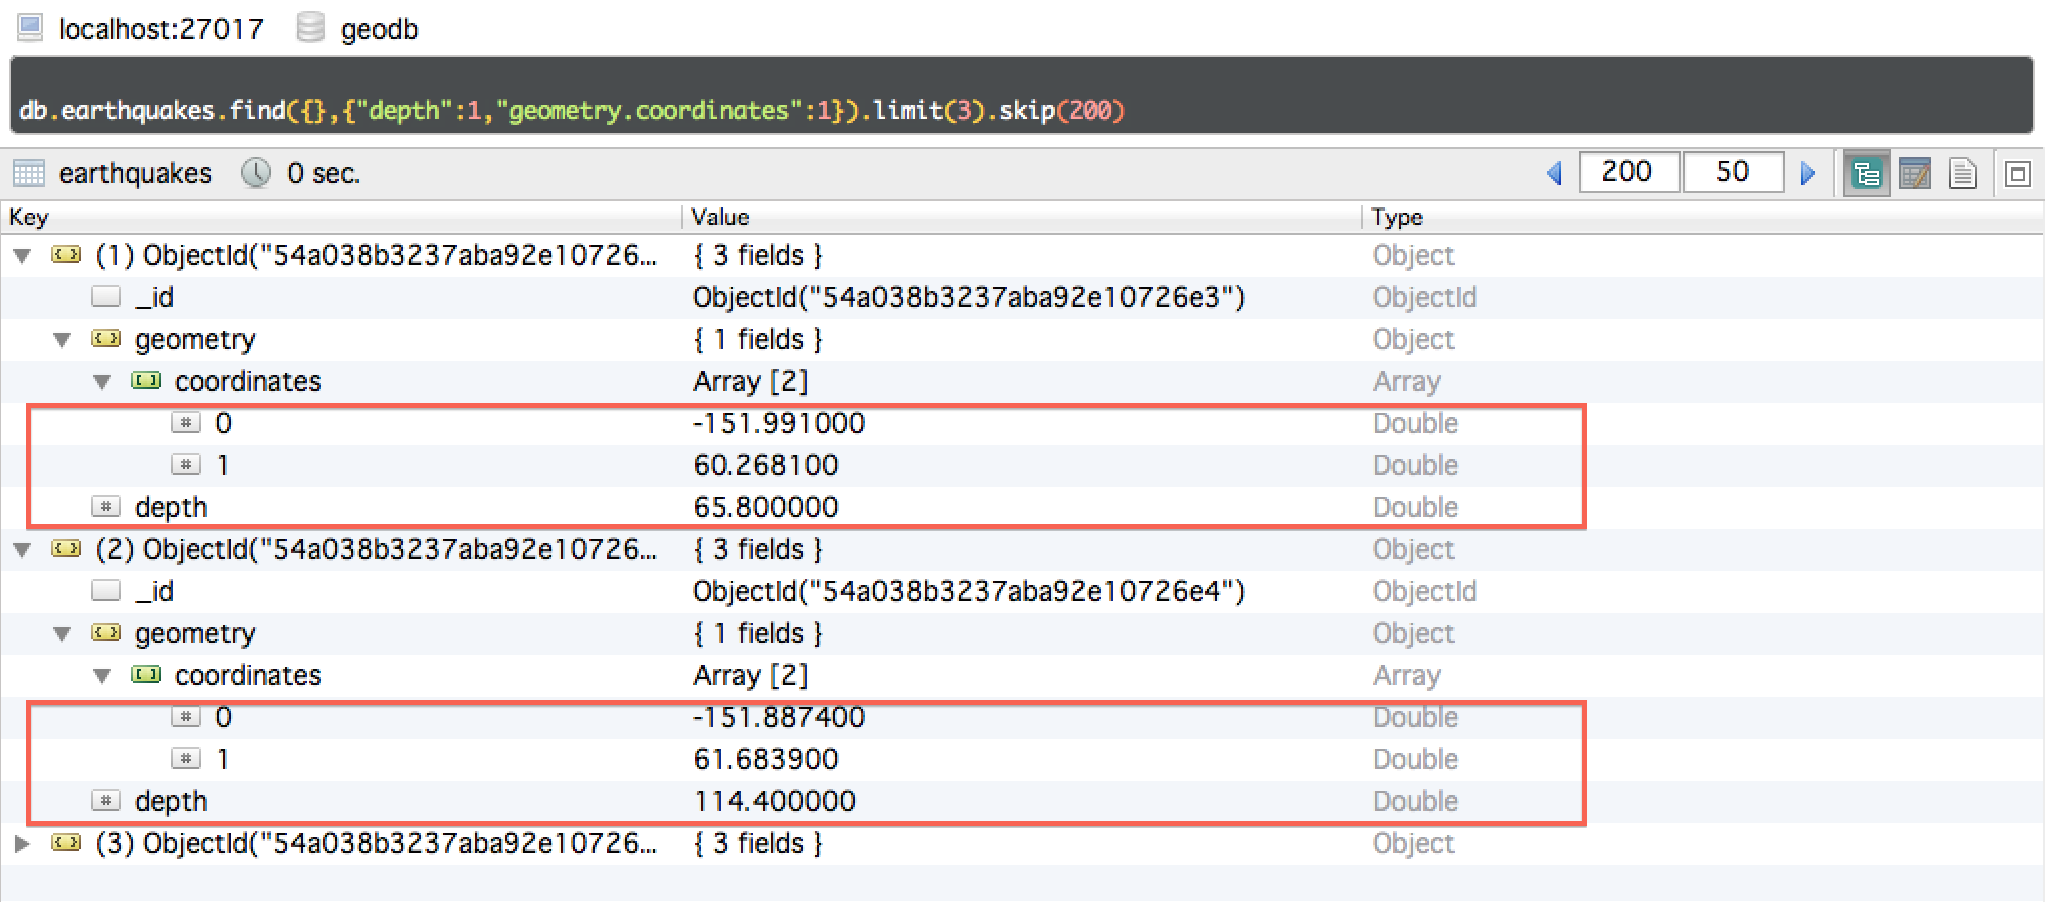
\includegraphics[scale=0.4]{img/depth.png}
    \caption{...find({},{"depth": 1, "geometry.coordinates": 1}).limit(3).skip(200)}
    \end{figure}

\subsection{Indexation géographique}
    MongoDB propose plusieurs types d'index, dont les "géospacial Indexes". Ils permettent de gérer des informations sur plusieurs dimensions (coordonnées, distance, position...). Il y en a notament un index pour les coordonées cartésienne et un autre pour les sphériques. L'index demandé est de type 2d.
    
    \par Ce type d'index prend en charge les coordonnées plannes  et ne supporte pas l'utilisation d"objet GeoJSON (contrairement à 2dsphere). Il prend comme argument le champ support de l'index et les options min, max bits. Par défaut mongodb considère les valeurs commes des longitudes et latitudes, elles vont donc de -190 à 190. Si une valeur sort de se cette fourchette mongodb renvoie un erreur. 
    
    \par Avant de créer l'index on vérifie donc que le jeux de données respecte bien cette convention avec les reqêtes suivantes : \newline
    \begin{tt} db.earthquakes.find({"geometry.coordinates": {\$gt: 10}}).count() \end{tt} \newline 
    \begin{tt} db.earthquakes.find({"geometry.coordinates": {\$lt: 10}}).count() \end{tt} \newline
    
    Le résultat est zero, les données sont adaptées, on ne préscise donc pas d"option.
    \begin{lstlisting}[language=Mongo, caption=]    
    db.earthquakes.ensureIndex({"geometry.coordinates": "2dsphere"})
    \end{lstlisting}
    
\newpage

    On peut alors requêter sur ce champs en utilisant des fonctions géométriques proposées par mongodb comme: \$geoIntersects, \$geoWithin, \$near. Exemple, exécuter une requête qui cherche les tremblements de terre
proche de la position -3.984,48.724 

    \begin{lstlisting}[language=Mongo, caption=]    
    db.earthquakes.find({
        "geometry.coordinates":
        {
            $near : [-3.984, 48.724],
            $maxDistance: 1000
        }
    });
    \end{lstlisting}
    
\section{Replication}

    \subsection{un maitre avec un ou plusieur esclaves}
    \par L'une des porpriétés de mongodb est sa capacité à gérer des duplicas pour offrire une base de donnée plus persistante. Une copie des données est alors faites sur un autre server. Mongodb est un système actif/passif\textsuperscript{6}, ses différnents noeuds portent un statut maître ou esclave.
    
    \par Pour simmuler les différents noeuds on utilise les ports d'une machine locale que l'on passe au démon. \begin{tt}mongo\end{tt} tout en indiquant le statu du noeud. On récupère quelques lignes de prompte intéressantes.
    \begin{itemize}
        \item Lancement du maître: \newline
        \begin{tt} mongod --master --dbpath .../data/master -port 27016 \end{tt}
        \item Premier esclace: \newline
        \begin{tt} mongod --slave --source localhost:27016 --dbpath .../data/slave -port 27018\end{tt}
        \item Deuxième esclave: \newline
        \begin{tt} mongod --slave --source localhost:27016 --dbpath .../data/slave2 -port 27020\end{tt}
    \end{itemize} 

    \begin{lstlisting}[language=JSON, caption= Prompt renvoyé par le noeud maître]


mongod --master --dbpath ~/Lmdapp/data/mongodb/data/master -port 27016
2015-01-17 [initandlisten] db version v2.6.6
[ ... ]
2015-01-17 [initandlisten] waiting for connections on port 27016
[ ... ]
2015-01-17 [clientcursormon]  connections:0
2015-01-17 [initandlisten] connection accepted from 127.0.0.1:50358 #1 (1 connection now open)
2015-01-17 [slaveTracking] build index on: local.slaves properties: { v: 1, key: { _id: 1 }, name: "_id_", ns: "local.slaves" }
[ ... ]
2015-01-17 [clientcursormon]  connections:1
2015-01-17 [initandlisten] connection accepted from 127.0.0.1:50731 #2 (2 connections now open)
2015-01-17 [slaveTracking] build index on: local.slaves properties: { v: 2, key: { _id: 2 }, name: "_id_", ns: "local.slaves" }
[ ... ]

\end{lstlisting}

    
            {\let\thefootnote\relax\footnotetext{
                \textsuperscript{6}Attention, le model mongo est assez controversé, exemple:\newline
                Evaluation sévère de mongo sur le post: \textit{\href{https://aphyr.com/posts/284-call-me-maybe-mongodb}{Call me maybe: MongoDB by aphyr}} \newline
                "...Mongo, un choix plus User firendly que résistant.": \textit{\href{http://bigdatahebdo.azurewebsites.net/episodes/2014/12/30/EP09_Mongodb/}{Tugdual Grall, au Talk BigDataHebdo.}
                }
            }
                
            
\newpage

    \par La base local donne des infos sur l'intence mongodb. l'instruction db.slaves.find() nous renvoies les propriétés des esclaves stokés dans mongodb. 
    
    \begin{lstlisting}[language=JSON, caption=]
> db.slaves.find().pretty()
{
	"_id" : ObjectId("54ba60891fd9ebd9f64c30ef"),
	"config" : {
		"host" : "127.0.0.1:50358",
		"upgradeNeeded" : true
	},
	"ns" : "local.oplog.$main",
	"syncedTo" : Timestamp(1421501959, 1)
},
{
	"_id" : ObjectId("54ba6df131f0c24be9fe3bb0"),
	"config" : {
		"host" : "127.0.0.1:51059",
		"upgradeNeeded" : true
	},
	"ns" : "local.oplog.$main",
	"syncedTo" : Timestamp(1421504048, 1)
}

    \end{lstlisting}
    
\begin{tabularx}{14cm}{|c|p{3cm}|X|}
    \hline
    1 & "host" & Nom et port du noeud esclave. \\
    \hline
    2 & "upgradeNeeded" & Etat de la réplication des neuds. "False" si le neud est à jour. \\
    \hline
    3 & "ns" & Collection contenant les logs liés aux réplication \\
    \hline
    4 & "syncedTo" & Dernière date de sychronisation. \\
    \hline
\end{tabularx}

    \par
        Pour tester la réplication, sur le noeud maître on insert un nouveau document dans une nouvelle collection d'une base encore inexistante. Mongodb créer automatiquement la base puis la réplique sur les autres noeuds. On la retrouve en se connectant aux esclaves et en appliquant la méthode show dbs.

\subsection{Plusieur maîtres et un esclave}
    \par Dans cette organisation le travaille s'effectue dans le sens inverse. Au lieu de lancer des slaves avec une adresse sources et attendre l'écriture des documents local.slaves on lance les maîtres et on insert leur adresse dans la collection local.sources d'un slave: \begin{tt}  db.sources.insert(host:"ip.a.dre.ss:port")\end{tt} \newline
 Une fois insérée la connection s'effectue et les documents se complètent avec l'\_id et la date du dernier update. On retrouve alors les collections des maîtres sur le neud esclave. Il est également possible de présciser dans les documents local.sources les collections à récupérer avec l"option "only".
    \par On retrouve en suite l'adresse slave dans la collection local.slave des maîtres. Chaque document ajouté est recopié.  
    
    
\section{Le sharding ou partitionement}

    MongoDB en plus de dupliquer les données propose également de les fragmenter et les répartire sur des noeuds distincts. Il est alors possible séparer une base en méttant les collections sur des machines différentes (scaling vertical). Ou disposer d'une partie des documents de toutes les collestions sur chaque noeuds (scaling horizontale).\newline
Pour cette partie on va créer un server de configuration et deux servers de shard: \newline
\begin{tt}
    mongod --port 27022 --dbpath .../data/config -configsvr \newline
    mongod --configdb localhost:27022 --port 27021 --chunkSize 1 \newline
    mongod --port 27023 --dbpath .../data/shard0 –shardsvr \newline
    mongod --port 27024 --dbpath .../data/shard1 --shardsvr \newline
\end{tt}

    L"oprtion --chunkSize donne une taille maximal aux collections. par défauts elles sont de 64 bits. En réduisant les tailles des collections on partionne plus rapidement.

    En se connnectant au controlleur on accède à un shell mongos (mongodb Shards). Une instance mongo qui permet la configuration des shards. Après la connection à admin, et le lancement de la commande: \newline
    \begin{tt}db.runCommand(\{ addshard:"adress:port",allowLocal:true\})\end{tt} \newline
On retrouve les shards que l'on a lancé dans la collection: config.shards:
\begin{lstlisting}[language=JSON, caption=]
mongos> use config 
switched to db config 
mongos> db.shards.find() 
{ "_id" : "shard0000", "host" : "localhost:27023" }
{ "_id" : "shard0001", "host" : "localhost:27024" }
\end{lstlisting} 

Pour la suite du TP on créer la base de donnée phone et on autorise le sharding de cette base avec la commande \begin{tt}db.runCommande({enablesharding:"base"})\end{tt}. On définit en suite la fonction qui génère les documents de la bases phones. 

\begin{block}{Remarque} Pour bien comprendre la diffusions des actions depuis le controlleur on se plug au mongos via RoboMongo. En faisant un .count() on retrouve 200 000. Puis en cosole on constate l'exitance des bases et collections sur les serveurs shards. On trouve respectivement sur les ports 27023 et 27024: 94627 et 105373 docs.\newline
(105373 + 94627 = 200 000)
\end{block}

\begin{block}{Vérificatio} Les testes demandés reviennent exactement à la remarque préscédente.
\end{block}


\section{Administration et sécurité}

    \subsection{Backup}
    \par Dans cette partie on découvre les commandes \begin{tt}mongodump\end{tt} et \begin{tt}mongorestore\end{tt} qui permettent respectivement de sauvegader et rétablir une ou plusieur bases de données (celon les options). Un dump de l'instence mongo donne une collection et son system.indexes au format .bson et fichier de metta données au format .json.
    
    \begin{block}{Note} Le démon mongod doit être lancé pour passer ces commandes.
    \end{block}
    
\subsection{Authetification}
    \par Dans cette partie la démarche indiquée est dépréciée. Connection à la base de donnée admin (use admin) et utilisation de la méthode .addUser(). A la place il est conseillé de créer un document de la manière suivnate. 

\begin{lstlisting}[language=JSON, caption=Création d"un user]
use admin
db.createUser(
  {
    user: "siteUserAdmin",
    pwd: "password",
    roles: [ { role: "userAdminAnyDatabase", db: "admin" } ]
  }
)
\end{lstlisting}
    
\newpage

\section*{\center{Annexe}}
    
    \subsection*{SQL to Mongodb, avec Node.js\textsuperscript{7}}

\par Une des problématiques apportées par les technos NoSQL est la conversion des anciennes base rellationnelles. Pour les petits acteurs du web qui passent sur des architechtures scalables avec des languages serveur comme node, la migration s'accompagne souvent d'un changement de base de données.

\par Bien que mongoDB ai son propre module node\textsuperscript{8} je propose ici un module concurrent \textbf{mongoose} \textsuperscript{9} qui lui nécessite la création d'un schéma. Le cas d'utilisation est simple: Si on recopie une une base SQL, il est plus simple de crée un shéma avant de la pousser dans Mongo.

\par Je propose donc le code suivant qui peut être lancé de la manière suivante:\newline
\begin{tt} > Node bank.js \end{tt} Le but est de pouvoir insérer dans mongoDB un export au format .Json d'une base MySQL, exemple:

\begin{lstlisting}[language=JSON, caption=Une ligne de l'export.]
{"Bid":"982","account_number":982,"balance":16511,"firstname":"Buck","lastname":"Robinson","age":24,...,"email":"buckrobinson@calcu.com"}
\end{lstlisting}

\begin{lstlisting}[language=JavaScript, caption=SQL to MongoDb avec le module Mongoose.]
mongoose = require('mongoose'); //import du module mongoose
fs = require('fs');            //

mongoose.connection.on('error', function(){// si il a une erreur.
  console.log('Failed to Connect to the BDD');
});

mongoose.connection.on('open', function(){// a la connection
  console.log('Connection to the BDD');
});

mongoose.connect('mongodb://localhost/bank'); // mongo> use bank

var count_model = mongoose.Schema({ //definition du schema
  'Bid':String,
  'account_number':Number,
  'balance':Number,
  'firstname':String,
  'age':Number,
  '...'
  'state':String
});

//Array ---> mongoose.model.Object
var account = mongoose.model('account', count_model);
console.log('Building Schema');

fs.exists('./accounts.json', function (exists) {
  //Si le fichier existe, L'ouvrire et Le lire
  fs.readFile('./accounts.json', function(err, data){
    var bank = JSON.parse(data);
    bank.forEach(function(d){
      var row = new account(d);
      row.save(function (err) {
        if(err)console.log('Inserting Error!');
      });
    });
  });
});
\end{lstlisting}

{\let\thefootnote\relax\footnotetext{\textsuperscript{7} \textit{\href{http://nodejs.org}{http://nodejs.org}}}}
{\let\thefootnote\relax\footnotetext{\textsuperscript{8} \textit{\href{http://mongodb.github.io/node-mongodb-native/}{Native Node module for MongoDB}}}}
{\let\thefootnote\relax\footnotetext{\textsuperscript{9} \textit{\href{http://mongoosejs.com}{Mongoose: mongodb object modeling for node.js}}}}
{\let\thefootnote\relax\footnotetext{\textsuperscript{10} \textit{Retrouvez l'exemple complet{\href{https://github.com/bly2k/files/blob/master/accounts.zip?raw=true}{ \textbf{ici}}.}}}

\newpage




    
\newpage

    
\subsection*{Map / Reduce avec Pymongo\textsuperscript{11}}

\par Pymongo est une dépendence python qui permet de s'adrésser à mogodb. Une fois L'instence mongo lancée L'import de ce module permet la connection et donne accès à des fonctions mongo.

\begin{tt} >>>>>> Import mongo\end{tt}

\par Pour faire un exemple on propose de reprendre la fonction map reduce de pymongo appliquée à la base de lapin de la partie 9. Pour lancer le script:

\begin{tt} > python mapredbunny.py\end{tt}

\lstset{language=python}
\begin{lstlisting}
##########################################################
#     EXEMPLE DE MAP / REDUCE SUR MONGODB                #
##########################################################

# Import du connecteur et du traducteur bson #
import pymongo
from bson.code import Code # Traduction du code Js compris par mongodb #

# Connection a la bonne BDD #
db = pymongo.MongoClient().lapins 

# ecriture du mappeur #
mapp = Code(""" 
            function() {
                this.regime.forEach(function(r){
                    emit(r,1);
                });
            }
            """)

# ecriture du reduceur #
red = Code(""" 
            function(key, tab) {
                var sum = 0;
                for(var i; i < tab.length - 1; i++){
                    sum += values[i];
                }
                return sum;
            }

            """)

# Lancement de l'agregation #
res = db.france.map_reduce(mapp, red, "mapred_bunny", query={"genre":"h"})
#
Le resultat est disponible
dans la collection "mapred_bunny"
#
\end{lstlisting}

\par La collection retour est une suite de document contenant: un nom d'alliment et le nombre de lapins mâles qui en mange. Ce n'est pas très util car ce n'est qu'un exemple. Il faut s'imaginer que la donnée est maintenant bien agrégée pour réaliser de super grafiques sur le régime des lapins de la collection france.

{\let\thefootnote\relax\footnotetext{\textsuperscript{11} \textit{{\href{http://api.mongodb.org/python/current/?_ga=1.152073017.1419368140.1410728889}{ API du connecteur "pymongo"}.}}}
 
    
    \subsection*{Sources}
Le code source de ce rapport est normalement disponible sur: \textit{ \href{https://github.com/DivLoic/TP-Mongodb}{https://github.com/DivLoic/TP-Mongodb}}. 
    
\end{document}

